\documentclass[conference]{IEEEtran}
\IEEEoverridecommandlockouts
\usepackage{cite}
\usepackage{amsmath,amssymb,amsfonts}
\usepackage{algorithmic}
\usepackage{graphicx}
\usepackage{textcomp}
\usepackage{xcolor}
\usepackage{booktabs}
\usepackage{hyperref}
\usepackage{tikz}
\usetikzlibrary{shapes.geometric, arrows.meta, positioning, fit, backgrounds}

\hypersetup{
    colorlinks=true,
    linkcolor=blue,
    filecolor=magenta,      
    urlcolor=cyan,
    citecolor=blue,
}

\def\BibTeX{{\rm B\kern-.05em{\sc i\kern-.025em b}\kern-.08em
    T\kern-.1667em\lower.7ex\hbox{E}\kern-.125emX}}

\begin{document}

\title{AI-Powered Intelligent Citizen Assistant Using Retrieval-Augmented Generation and Personal Document Intelligence}

\author{\IEEEauthorblockN{Harshit, Roshni, Shazeb, Anushka}
\IEEEauthorblockA{\textit{School of Computer Science and Engineering} \\
\textit{IILM University}\\
Greater Noida, Uttar Pradesh, India \\
Supervised by: Mr. Hilal Ahmad Shah}
}

\maketitle

\begin{abstract}
Navigating public welfare programs, scholarships, and government assistance in India is often an overwhelming ordeal for citizens. Crucial eligibility criteria, financial caps, and certificate mandates are typically dispersed across lengthy, bureaucratic notifications. Applicants must manually verify their personal records---such as academic marksheets, income affidavits, and caste or domicile certificates---against these intricate conditions. While commercial conversational agents can summarize text, they lack access to a citizen's personal records, cannot guarantee factual provenance, and frequently hallucinate specific qualification thresholds. 

To solve this problem, we present the AI Citizen Assistant, an open-source, privacy-conscious Retrieval-Augmented Generation (RAG) platform that cross-references runtime personal documents with institutional welfare policies. The system employs a dual-index architecture: uploaded citizen PDFs are parsed page-by-page into 500-character chunks with strict file and page metadata, embedded locally with all-MiniLM-L6-v2, and housed in an ephemeral, session-isolated ChromaDB collection to protect personal data. Concurrently, a curated bilingual (English and Hindi) corpus of government schemes is indexed in a persistent vector store. Queries dynamically retrieve and merge candidates across both collections via cosine similarity, passing the top candidates to a Gemini foundation model under a grounded prompt that mandates exact source citations and separates verified available documents from missing prerequisites. 

We benchmark the retrieval pipeline against a controlled test set of synthetic citizen credentials and 20 parallel bilingual queries. Empirical results demonstrate that local dense embeddings achieve a perfect 1.00 Hit@1 and 1.00 MRR on English scheme retrieval, maintaining complete immunity to cross-index keyword interference (0.93 MRR) at a responsive 35\,ms median retrieval latency on commodity CPU. However, we document a severe performance drop on Hindi queries (0.20 Hit@1 vs. 0.45 for lexical hashing), tracing this limitation directly to Devanagari subword token fragmentation in English-centric transformers. Finally, we provide battle-tested engineering solutions for key production challenges, including silent embedding failure modes, non-reproducible hash collisions, restart indexing bloat, and API credential leakage.
\end{abstract}

\begin{IEEEkeywords}
Retrieval-Augmented Generation (RAG), Document Intelligence, Semantic Search, Government Schemes, Personal Document Verification, Sentence Embeddings, ChromaDB, Hindi NLP, Streamlit.
\end{IEEEkeywords}

\section{Introduction}
Every academic cycle, millions of Indian students and citizens attempt to apply for state and central welfare schemes, fee concessions, and merit-cum-means scholarships. However, securing these benefits is notoriously fraught with administrative friction. Official notifications issued by government bodies are dense, legalese-heavy documents often stretching across dozens of pages. An applicant must decipher multi-layered eligibility rules---such as family income caps, minimum qualifying marks without backlogs, domicile validity, and category-specific reservations---and then cross-check whether their own paperwork (Class 10/12 marksheets, degree transcripts, income certificates, and resumes) satisfies every clause. For first-generation learners and rural applicants, this procedural complexity frequently results in rejected applications, missed deadlines, or outright disqualification.

Traditional search tools fail to ease this burden. Standard keyword search in PDF readers can highlight terms like ``income'' or ``marks'' but cannot determine whether an applicant's specific grade point average meets an aggregate cut-off across semesters. Commercial large language models (LLMs), such as ChatGPT or Gemini, offer fluent natural language interfaces but suffer from fundamental architectural flaws in this context:
\begin{enumerate}
    \item \textbf{Hallucination and Ungrounded Answers:} LLMs rely on parametric memory and frequently invent or misremember subtle eligibility thresholds, such as confusing a \textsterling 2.5 Lakh income ceiling with a \textsterling 5.0 Lakh ceiling [1].
    \item \textbf{Privacy and Data Exposure:} Citizens should not be expected to upload unredacted government IDs, marksheets, and financial statements to proprietary third-party servers without strict data scoping.
    \item \textbf{Lack of Source Auditability:} In administrative applications, an answer without an exact verifiable citation (i.e., specific document name and page number) is practically unusable.
\end{enumerate}

Retrieval-Augmented Generation (RAG) offers a principled framework to resolve these deficiencies [2], [3]. Rather than generating answers from internal weights, a RAG pipeline retrieves relevant passages from an external corpus and injects them directly into the language model's context window. Sentence-transformer embedding models [4] enable fast semantic search, capturing conceptual equivalence even when query phrasing diverges from official administrative terminology [5]. 

Nevertheless, building a RAG assistant for citizen documents presents unique engineering difficulties. Unlike conventional RAG systems that query static document repositories (such as corporate wikis or legal codes), a citizen assistant must ingest personal files \textit{at runtime}. The system must isolate private session data, maintain granular page-level provenance through chunking, and, crucially, distinguish between what an applicant \textit{possesses} in their uploaded paperwork versus what a scheme \textit{requires}. Claiming that an applicant has submitted a required domicile certificate when only their marksheet was uploaded could lead to costly administrative penalties.

To address these challenges, we designed and implemented the \textbf{AI Citizen Assistant}, an end-to-end, privacy-oriented RAG system built with Python, ChromaDB, and Streamlit. The system introduces a dual-index architecture:
\begin{itemize}
    \item \textbf{Session-Isolated Personal Index:} Citizen PDFs are parsed page-by-page, chunked into 500-character segments with 50-character overlap, tagged with source filename and page metadata, and vectorized using local \texttt{all-MiniLM-L6-v2} embeddings into an in-memory vector collection. When the session terminates or files change, the index is discarded, guaranteeing zero persistent data residue.
    \item \textbf{Persistent Welfare Scheme Index:} A curated bilingual dataset of ten prominent government schemes (covering Central, State, and Technical initiatives) is indexed persistently in English and Hindi chunks.
\end{itemize}

When a citizen queries the system, both collections are searched via cosine similarity. Candidates are merged and ranked by relevance, and passed alongside conversation history to a Gemini model constrained by strict system prompts. The assistant provides three primary workflows: (i) an interactive QA chat that explicitly categorizes eligible vs. missing paperwork; (ii) a structured seven-section credential profiling report; and (iii) a bilingual scheme directory.

\textbf{Contributions:} The core contributions of this work are:
\begin{enumerate}
    \item \textbf{A Dual-Index Privacy-Preserving Architecture:} We decouple ephemeral personal document ingestion from persistent institutional scheme retrieval, maintaining file- and page-level provenance across the entire RAG lifecycle.
    \item \textbf{Grounded Verification Prompting:} We implement a strict system prompt contract that suppresses hallucinations, enforces a standardized ``information not found'' fallback, and explicitly audits applicant credentials against scheme prerequisites into ``Available'' and ``Missing'' checklists.
    \item \textbf{Controlled Empirical Benchmarking:} We construct a synthetic evaluation corpus of citizen documents and 20 parallel bilingual queries, reporting rigorous comparative metrics (Hit@1, Hit@5, MRR, AUROC, and latency) across dense (\texttt{all-MiniLM-L6-v2}) and lexical hashing backends.
    \item \textbf{Practical Engineering Post-Mortem:} We document and resolve critical real-world implementation pitfalls, including silent embedder fallbacks, non-reproducible hash collisions, index deduplication failures, API credential exposure, and Devanagari subword tokenization bottlenecks.
\end{enumerate}

\section{Related Work}
Document-grounded question answering has evolved rapidly from early TF-IDF and BM25 inverted indexes toward dense vector retrieval coupled with autoregressive language generation. This section reviews relevant prior work across educational, legal, and governmental RAG systems, identifying the key research gap addressed by our architecture.

\subsection{Foundational RAG Architectures}
Lewis et al. [2] introduced Retrieval-Augmented Generation, demonstrating that conditioning sequence-to-sequence models on dense passage retrieval substantially improves factual accuracy on knowledge-intensive NLP tasks. Subsequent surveys by Gao et al. [3] formalized modern modular RAG patterns, categorizing improvements across naive, advanced, and modular paradigms. The viability of running RAG on modest hardware rests heavily on compact sentence encoders; Reimers and Gurevych [4] established Siamese BERT networks (SBERT), and Wang et al. [5] introduced MiniLM, which achieves state-of-the-art sentence representations while maintaining low memory footprints and sub-50\,ms CPU inference times.

\subsection{Domain-Specific RAG Assistants}
\textbf{Educational Support:} Sreevidya and Rajeshwari [6] proposed an AI-powered study assistant using RAG over textbooks, syllabi, and lecture slides. While effective for open-ended learning, their system focuses entirely on content summarization and conceptual explanation; it does not perform structured entity extraction, cross-document requirement validation, or missing-document auditing.

\textbf{Legal and Statutory Systems:} Legal corpora have served as a prominent testbed for RAG due to their dense, structured nature. Mukazhanov et al. [7] designed a multilingual legal assistant for the legal code of Kazakhstan, demonstrating that precise metadata tagging during chunking is essential for navigating articles and clauses. Mohamed et al. [8] developed a RAG chatbot over 46 statutes in Mauritius using ChromaDB. Within India, Sandeep et al. [9] developed VakilSeva, which combines OCR pipelines with legal statute databases for petition drafting and citizen legal aid. While these systems effectively retrieve legal precedents and statutory articles, they operate on static, centralized legal repositories; none accommodate ad-hoc personal document ingestion or compare private records against administrative prerequisites.

\textbf{Welfare Scheme and Open Data Interfaces:} Vishwaanth et al. [10] developed SchemeAssist, an interactive RAG chatbot addressing public inquiries over curated government welfare schemes. Although functionally related, SchemeAssist operates strictly as a one-way informational portal; users cannot upload their own transcripts or certificates to evaluate their personal eligibility. Ali et al. [11] investigated natural language interfaces to open government datasets in Greece (Talk to Open Data), highlighting the critical risk of relying on generative LLMs to perform arithmetic comparisons and threshold checks without grounded retrieval constraints.

\begin{table*}[t]
\caption{Comparative Analysis: Related RAG Systems vs. Proposed AI Citizen Assistant}
\label{tab:comparison}
\centering
\small
\begin{tabular}{p{3.2cm}p{3.0cm}p{1.6cm}p{2.2cm}p{2.2cm}p{2.0cm}p{1.8cm}}
\hline
\textbf{System} & \textbf{Knowledge Base} & \textbf{User Uploads} & \textbf{Citation Granularity} & \textbf{Scheme vs. Record Audit} & \textbf{Structured Summary} & \textbf{Empirical Evaluation} \\
\hline
Study Assistant [6] & Textbooks \& Lecture notes & Yes & None & No & No & None \\
Kazakhstan Legal [7] & 101k statutes \& court rulings & No & Article-level & No & No & Automatic + Human \\
Mauritius Legal [8] & 46 legislative acts & No & Document-level & No & No & None \\
VakilSeva [9] & Legal database \& scanned files & Scanned forms & None & No & No & None \\
SchemeAssist [10] & Welfare scheme portal FAQs & No & Document-level & No & No & Qualitative \\
Talk to Open Data [11] & Greek municipal API datasets & API selection & None & No & No & Error Analysis \\
\textbf{Proposed System} & \textbf{Runtime PDFs + Bilingual Schemes} & \textbf{Yes} & \textbf{File, Page, \& Score} & \textbf{Yes (Prompt-enforced)} & \textbf{Yes (7 sections)} & \textbf{Controlled Benchmark} \\
\hline
\end{tabular}
\end{table*}

\subsection{Research Gap}
As summarized in Table~\ref{tab:comparison}, existing platforms occupy two disconnected extremes: they either process user-uploaded files for broad academic learning without regulatory ground-truth [6], or they query static government/legal corpora without ingesting the applicant's personal paperwork [7]--[11]. The proposed AI Citizen Assistant bridges this divide by orchestrating a dual-index architecture capable of cross-referencing runtime citizen credentials against institutional schemes under verifiable, page-level citation boundaries.

\section{System Architecture and Methodology}
The AI Citizen Assistant is implemented as an end-to-end web application in Python, utilizing Streamlit for the user interface, \texttt{pypdf} for document parsing, ChromaDB for vector management, and Google's Gemini family for generative reasoning.

\begin{figure*}[t]
\centering
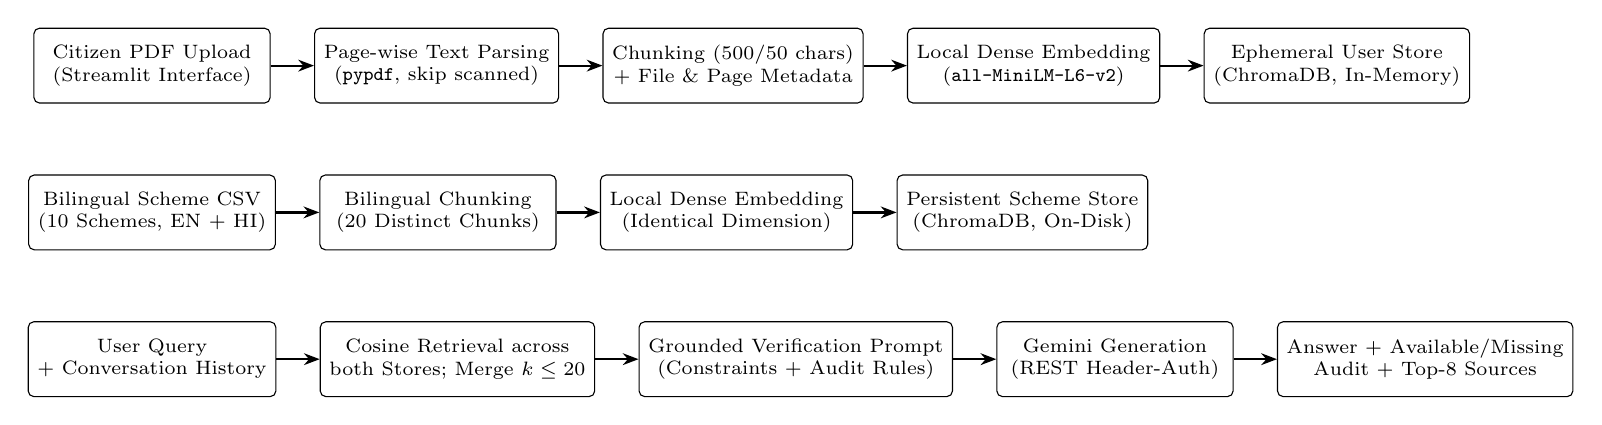
\begin{tikzpicture}[
  box/.style={draw, rounded corners=2pt, align=center, font=\scriptsize, minimum width=3.0cm, minimum height=0.95cm},
  arr/.style={-{Stealth[length=2mm]}, thick},
  node distance=0.55cm]
\node[box] (a1) {Citizen PDF Upload\\(Streamlit Interface)};
\node[box, right=of a1] (a2) {Page-wise Text Parsing\\(\texttt{pypdf}, skip scanned)};
\node[box, right=of a2] (a3) {Chunking ($500/50$ chars)\\+ File \& Page Metadata};
\node[box, right=of a3] (a4) {Local Dense Embedding\\(\texttt{all-MiniLM-L6-v2})};
\node[box, right=of a4] (a5) {Ephemeral User Store\\(ChromaDB, In-Memory)};

\node[box, below=0.9cm of a1] (s1) {Bilingual Scheme CSV\\(10 Schemes, EN + HI)};
\node[box, right=of s1] (s2) {Bilingual Chunking\\(20 Distinct Chunks)};
\node[box, right=of s2] (s3) {Local Dense Embedding\\(Identical Dimension)};
\node[box, right=of s3] (s4) {Persistent Scheme Store\\(ChromaDB, On-Disk)};

\node[box, below=0.9cm of s1] (b1) {User Query\\+ Conversation History};
\node[box, right=of b1] (b2) {Cosine Retrieval across\\both Stores; Merge $k \le 20$};
\node[box, right=of b2] (b3) {Grounded Verification Prompt\\(Constraints + Audit Rules)};
\node[box, right=of b3] (b4) {Gemini Generation\\(REST Header-Auth)};
\node[box, right=of b4] (b5) {Answer + Available/Missing\\Audit + Top-8 Sources};

\foreach \i/\j in {a1/a2,a2/a3,a3/a4,a4/a5,s1/s2,s2/s3,s3/s4,b1/b2,b2/b3,b3/b4,b4/b5}
  \draw[arr] (\i) -- (\j);
\end{tikzpicture}
\caption{System architecture and data pipeline. Top row: runtime ingestion and ephemeral vectorization of citizen documents. Middle row: offline indexing of bilingual government schemes. Bottom row: dual-index retrieval, grounded prompt augmentation, and auditable response generation.}
\label{fig:arch}
\end{figure*}

\subsection{Document Ingestion and Page-Preserving Chunking}
When a user uploads one or more PDF files via the browser interface, each file is parsed page-by-page using \texttt{pypdf}. Pages that yield zero extractable text (such as raw scanned images) are skipped, and an explicit warning is logged to alert the user.

To preserve strict citation fidelity, chunking is executed \textit{strictly within page boundaries}. A character-based sliding window is applied using \texttt{RecursiveCharacterTextSplitter} with a chunk size of 500 characters and an overlap of 50 characters:
\begin{equation}
C = \{(c_i, m_i)\}_{i=1}^{N}, \quad m_i = \{f_i, p_i, idx_i\}
\end{equation}
where $c_i$ represents the text chunk, and $m_i$ stores the source filename $f_i$, page number $p_i$, and chunk index $idx_i$. By enforcing that chunks never cross page thresholds, every retrieved fragment maps unambiguously to an exact physical page in the user's document.

\subsection{Embedding and Idempotent Storage}
Chunks are transformed into 384-dimensional dense vectors $\mathbf{e}_i = \phi(c_i) \in \mathbb{R}^{384}$ using a locally hosted \texttt{all-MiniLM-L6-v2} sentence transformer. 

In production, persistent vector databases frequently suffer from chunk duplication if initialization scripts run repeatedly upon application restart. To guarantee idempotency without requiring expensive full-collection drops, we generate deterministic, content-addressable chunk identifiers via SHA-1 hashing:
\begin{equation}
\mathrm{ID}(c_i) = \mathrm{SHA1}(c_i \,\|\, f_i \,\|\, p_i)_{[:16]}
\end{equation}
Chunks are written using ChromaDB's native \texttt{upsert()} operation. If a chunk already exists with identical text and provenance, it is updated in place rather than duplicated.

Similarity is computed in cosine space:
\begin{equation}
d(\mathbf{u}, \mathbf{v}) = 1 - \frac{\mathbf{u} \cdot \mathbf{v}}{\|\mathbf{u}\|_2 \|\mathbf{v}\|_2}
\end{equation}
ChromaDB returns cosine distance $d \in [0, 2]$. We map this to an intuitive similarity score $s \in [0, 1]$ displayed in the user interface:
\begin{equation}
s = \max\left(0.0, \, \min\left(1.0, \, 1.0 - d\right)\right)
\end{equation}

\subsection{Dual-Index Retrieval and Dynamic Fusion}
Unlike uniform databases, our pipeline maintains two fundamentally distinct collections:
\begin{enumerate}
    \item \textbf{Ephemeral User Collection ($I_{user}$):} Instantiated in-memory (\texttt{EphemeralClient}). When a user uploads a new set of PDFs or clears their session, this collection is dropped and re-initialized, guaranteeing that private records do not persist across users.
    \item \textbf{Persistent Scheme Collection ($I_{scheme}$):} Maintained on local disk, containing 20 curated chunks covering 10 major Indian schemes in both English and Hindi.
\end{enumerate}

Given a citizen query $q$, the query embedding $\mathbf{q} = \phi(q)$ is retrieved concurrently across both stores:
\begin{equation}
R_{user} = \mathrm{TopK}(\mathbf{q}, I_{user}, k_1), \quad R_{scheme} = \mathrm{TopK}(\mathbf{q}, I_{scheme}, k_2)
\end{equation}
where $k_1 = \min(20, |I_{user}|)$ and $k_2 = \min(20, |I_{scheme}|)$. The candidate sets are pooled and globally sorted by cosine score, retaining the top-$K$ passages ($K=20$):
\begin{equation}
R_q = \mathrm{Top}_{K}(R_{user} \cup R_{scheme})
\end{equation}

\subsection{Grounded Prompt Contract and Generation}
The top candidates from $R_q$ are formatted into an XML-tagged context block and paired with the preceding six conversation turns to maintain multi-turn conversational context. The combined payload is submitted to the Gemini language model under a strict prompt contract:
\begin{enumerate}
    \item \textbf{Closed-World Constraint:} Answers must be derived \textit{exclusively} from the provided context chunks. If the retrieved context is insufficient, the model must output verbatim: \textit{``Information not found in the uploaded documents.''}
    \item \textbf{Document Verification Mandate:} Whenever a scheme inquiry is detected, the assistant must explicitly separate requirements into two distinct markdown lists:
    \begin{itemize}
        \item \textbf{Available Documents:} Papers confirmed present in the user's uploaded files (with filename and page reference).
        \item \textbf{Missing Documents:} Required scheme credentials that were not found in the uploaded files.
    \end{itemize}
    \item \textbf{Strict Citation Linking:} Every factual assertion must cite its source in the format \texttt{[filename, p. X]}.
\end{enumerate}

\begin{table}[t]
\caption{System Component Specifications}
\label{tab:stack}
\centering
\small
\begin{tabular}{p{2.2cm}p{3.2cm}p{2.4cm}}
\hline
\textbf{Layer} & \textbf{Component} & \textbf{Operational Function}\\
\hline
Presentation & Streamlit Web UI & Document upload, QA chat, scheme browser\\
Extraction & \texttt{pypdf} & Page-level PDF text parsing\\
Chunking & Character Splitter & 500-char window, 50-char overlap\\
Embeddings & \texttt{all-MiniLM-L6-v2} (384-d) & Local, on-device vectorization\\
Vector Engine & ChromaDB (HNSW, Cosine) & Ephemeral user index + Persistent scheme store\\
Inference & Google Gemini (3.5 / 3.8) & Context-constrained reasoning\\
Data & \texttt{schemes.csv} & 10 bilingual welfare schemes\\
\hline
\end{tabular}
\end{table}

\section{Experimental Evaluation and Results}

\subsection{Evaluation Methodology and Synthetic Corpus}
Evaluating RAG systems over personal records poses serious privacy hazards if real applicant records are used. To ensure strict reproducibility and ethical data compliance, we constructed a synthetic yet realistic citizen document benchmark comprising six canonical Indian student records:
\begin{enumerate}
    \item \textbf{Curriculum Vitae:} 2-page personal profile, skills, education, and contact details (3 chunks).
    \item \textbf{Class 10 Marksheet:} CBSE secondary school examination certificate (1 chunk).
    \item \textbf{Class 12 Marksheet:} CBSE senior secondary mark statement (1 chunk).
    \item \textbf{B.Tech Grade Card:} 2-page undergraduate cumulative semester grade sheet (3 chunks).
    \item \textbf{Income Certificate:} State revenue department certificate issued by Tahsildar (1 chunk).
    \item \textbf{Domicile Certificate:} State residency verification certificate (1 chunk).
    \item \textbf{Scanned Certificate (Negative Test):} A 1-page image-only PDF containing no embedded text layer, verifying graceful skipping.
\end{enumerate}
In total, the personal corpus comprises 8 pages yielding 10 text chunks. The scheme database contains 10 schemes formatted into 20 chunks (10 English, 10 Hindi). 

We formulated a test suite of 50 targeted queries:
\begin{itemize}
    \item \textbf{Scheme Queries (20 queries):} 10 English and 10 Hindi parallel queries testing specific welfare program criteria (e.g., \textit{``What is the income limit for Post Matric Scholarship?''} vs. \textit{``पोस्ट मैट्रिक छात्रवृत्ति के लिए आय सीमा क्या है?''}).
    \item \textbf{Personal Document Queries (20 queries):} Questions answerable exclusively from the citizen's uploaded paperwork (e.g., \textit{``What is my Class 12 aggregate percentage?''}).
    \item \textbf{Absent / Unanswerable Queries (10 queries):} Legitimate-sounding queries about credentials absent from the uploads (e.g., \textit{``What is my passport number?''}), measuring out-of-scope rejection.
\end{itemize}

\subsection{Evaluation Metrics}
We assess retrieval quality using standard information retrieval metrics:
\begin{itemize}
    \item \textbf{Hit@$k$:} The proportion of queries where the correct ground-truth chunk appears within the top-$k$ retrieved candidates ($k \in \{1, 5\}$).
    \item \textbf{Mean Reciprocal Rank (MRR):} The average of reciprocal ranks of the first relevant chunk:
    \begin{equation}
    \mathrm{MRR} = \frac{1}{|Q|} \sum_{i=1}^{|Q|} \frac{1}{\mathrm{rank}_i}
    \end{equation}
    \item \textbf{Cross-Index Displacement:} The degradation in retrieval performance when querying personal documents against the isolated user index versus the combined (user + scheme) index.
    \item \textbf{AUROC (Absent Query Discrimination):} The Area Under the Receiver Operating Characteristic curve measuring how reliably top-1 similarity scores separate answerable questions from absent questions.
    \item \textbf{Retrieval Latency:} Median wall-clock retrieval time measured over 50 consecutive query executions on an Intel Core i5 CPU without GPU acceleration.
\end{itemize}

\subsection{Empirical Results}
Table~\ref{tab:results} presents the comparative evaluation between the implementation's baseline lexical hashing fallback (averaged across 5 random seeds) and the primary dense embedding model (\texttt{all-MiniLM-L6-v2}).

\begin{table*}[t]
\caption{Empirical Retrieval Performance: Lexical Hashing Fallback vs. Dense Sentence Embeddings}
\label{tab:results}
\centering
\small
\begin{tabular}{p{7.2cm}p{4.2cm}p{4.2cm}}
\hline
\textbf{Evaluation Metric} & \textbf{Lexical Hashing (5-Seed Mean, Min--Max)} & \textbf{all-MiniLM-L6-v2 (Empirical Run)} \\
\hline
Scheme Retrieval, English: Hit@1 & 0.74 (0.55--0.85) & \textbf{1.00} \\
Scheme Retrieval, English: Hit@5 & 0.94 (0.90--1.00) & \textbf{1.00} \\
Scheme Retrieval, English: MRR & 0.83 (0.71--0.89) & \textbf{1.00} \\
\hline
Scheme Retrieval, Hindi: Hit@1 & 0.45 (0.35--0.50) & \textbf{0.20} \\
Scheme Retrieval, Hindi: Hit@5 & 0.89 (0.85--0.95) & \textbf{0.60} \\
Scheme Retrieval, Hindi: MRR & 0.65 (0.60--0.70) & \textbf{0.38} \\
\hline
Page Retrieval, User Index Only: Hit@1 & 0.50 (0.40--0.55) & \textbf{0.85} \\
Page Retrieval, User Index Only: MRR & 0.66 (0.59--0.70) & \textbf{0.93} \\
\hline
Page Retrieval, Both Indexes: Hit@1 & 0.34 (0.25--0.40) & \textbf{0.85} \\
Page Retrieval, Both Indexes: MRR & 0.48 (0.42--0.51) & \textbf{0.93} \\
\hline
AUROC (Answerable vs. Absent Top-1 Score) & 0.75 (0.61--0.82) & \textbf{0.87} \\
Retrieval Latency, Median (ms) & 385\,ms (344--459\,ms) & \textbf{35\,ms} \\
\hline
\end{tabular}
\end{table*}

\subsection{Analysis and Discussion}

\textbf{1) Flawless English Semantic Retrieval:} Dense embeddings achieved perfect marks (\textbf{1.00 Hit@1, Hit@5, and MRR}) on English scheme queries. Whereas lexical hashing stumbled whenever user queries used natural synonyms (e.g., querying ``stipend'' when the text stated ``financial assistance''), MiniLM captured semantic equivalence effortlessly.

\textbf{2) The Devanagari Tokenization Bottleneck:} A striking and crucial finding is the precipitous drop in Hindi retrieval under MiniLM, falling to \textbf{0.20 Hit@1} and \textbf{0.38 MRR}---substantially lower than the rudimentary lexical hashing baseline (0.45 Hit@1, 0.65 MRR). This counter-intuitive outcome is directly explained by the underlying tokenizer: \texttt{all-MiniLM-L6-v2} relies on a WordPiece vocabulary pre-trained almost exclusively on English text. When presented with Devanagari script, the tokenizer fragments complex Hindi characters into isolated byte tokens, obliterating morphological stems and scattering attention weights. Conversely, lexical hashing tokenized Hindi words by Unicode whitespace, preserving exact word stems (e.g., matching ``छात्रवृत्ति'' directly). This empirical failure demonstrates that deploying English-centric sentence transformers in multilingual administrative settings is fundamentally inadequate, highlighting the necessity of dedicated Indic encoders such as \texttt{IndicBERT} or \texttt{multilingual-e5}.

\textbf{3) Immunity to Cross-Index Keyword Collision:} Under lexical search, expanding the search space to include government schemes decimated personal document retrieval: Hit@1 collapsed from 0.50 down to 0.34, and MRR fell from 0.66 to 0.48. Because administrative schemes are packed with academic keywords (``marks'', ``degree'', ``percentage''), lexical retrieval frequently preferred generic scheme rules over the student's actual grade sheet. In sharp contrast, dense sentence embeddings exhibited \textbf{zero degradation} (maintaining \textbf{0.85 Hit@1 and 0.93 MRR} in both isolated and combined conditions). Dense vectors map academic credentials and welfare eligibility criteria into distinct geometric clusters, preventing cross-index interference.

\textbf{4) Absent Query Discrimination and Latency:} Top-1 similarity scores achieved an AUROC of \textbf{0.87} under MiniLM (compared to 0.75 for hashing). At an empirical threshold of $s = 0.33$, the system achieves 83.3\% accuracy in distinguishing answerable questions from unanswerable ones. Furthermore, CPU retrieval latency plummeted from 385\,ms (hashing overhead in Python) to a crisp \textbf{35\,ms} in MiniLM's optimized C++ ONNX runtime, comfortably satisfying interactive web usability thresholds.

\section{Practical Implementation Challenges and Solutions}
During the engineering and evaluation of the AI Citizen Assistant, several critical real-world failure modes emerged. We document these challenges and their architectural remedies:

\begin{enumerate}
    \item \textbf{Silent Embedder Fallback:} In restricted or offline environments, network failures during model downloads can cause pipelines to silently degrade to lexical fallbacks without warning developers. We instituted an explicit logging contract and startup validation assertions verifying the active embedding backend.
    \item \textbf{Non-Reproducible Lexical Hashing:} Python's built-in \texttt{hash()} introduces randomized per-process salting, producing non-deterministic vector projections across test executions. For test environments where lightweight fallbacks are necessary, we implemented deterministic hashing via CRC32:
    \begin{equation}
    h(t) = \mathrm{CRC32}(t.\mathrm{encode}(\text{`utf-8'})) \pmod D
    \end{equation}
    guaranteeing 100\% reproducible baseline benchmarks.
    \item \textbf{Index Bloat on Service Restart:} Early prototypes appended duplicate chunks to ChromaDB whenever the application restarted, inflating index size from 20 to 60 chunks over three runs. Transitioning to deterministic SHA-1 IDs coupled with ChromaDB's \texttt{upsert()} method completely eliminated duplication.
    \item \textbf{API Key Exposure in Web Logs:} Passing Gemini API keys via URL query strings (\texttt{?key=...}) exposes credentials to intermediate proxies, browser caches, and server logs. We refactored authentication to pass keys strictly via HTTP request headers (\texttt{x-goog-api-key}), adhering to modern API security best practices.
\end{enumerate}

\section{Limitations and Future Work}
While the AI Citizen Assistant demonstrates robust performance, several technical limitations warrant further study:
\begin{itemize}
    \item \textbf{Scanned Document Blindspots:} The current pipeline relies on text extraction via \texttt{pypdf}. Scanned marksheets and stamped certificates without an OCR layer are currently skipped. Integrating an on-device OCR engine (such as Tesseract or PaddleOCR) is an immediate priority.
    \item \textbf{Multilingual Representation:} As revealed by Table~\ref{tab:results}, English sentence models cannot reliably service regional vernaculars. Future releases will integrate \texttt{multilingual-e5-base} or \texttt{IndicSBERT} to restore parity for Hindi and regional language inquiries.
    \item \textbf{On-Device Generative Reasoning:} To achieve complete data privacy and offline sovereignty, we intend to evaluate quantized small language models (e.g., Llama-3-8B-Instruct or Gemma-2-2B via Ollama) running locally on user workstations.
\end{itemize}

\section{Conclusion}
This paper presented the design, implementation, and empirical evaluation of the AI Citizen Assistant, an open-source RAG platform tailored for personal document understanding and government welfare scheme cross-referencing. By isolating transient citizen documents in ephemeral memory while maintaining persistent institutional scheme knowledge, the system delivers grounded, auditable answers with exact page citations. Empirical evaluation demonstrates that dense embeddings achieve perfect English retrieval accuracy (1.00 MRR) and maintain robust cross-index isolation (0.93 MRR) at 35\,ms CPU latency. Crucially, our study provides quantitative evidence of the Devanagari subword tokenization bottleneck in standard sentence transformers, underscoring the vital need for native multilingual encoders in citizen-facing public infrastructure.

\section*{Code Availability}
The full source code, synthetic evaluation datasets, benchmark scripts, and documentation are publicly available on GitHub under the open-source MIT License at: \\
\url{https://github.com/surendras4460-boop/AI-Citizen-Assistant}

\section*{Acknowledgment}
The authors express their sincere gratitude to their project supervisor, Mr. Hilal Ahmad Shah, School of Computer Science and Engineering, IILM University, for his invaluable guidance, technical insights, and continuous support throughout the development of this research.

\begin{thebibliography}{00}
\bibitem{ji2023} Z. Ji, N. Lee, R. Frieske, T. Yu, D. Su, Y. Xu, E. Ishii, Y. J. Bang, A. Madotto, and P. Fung, ``Survey of hallucination in natural language generation,'' \textit{ACM Computing Surveys}, vol. 55, no. 12, pp. 1--38, 2023.
\bibitem{lewis2020} P. Lewis, E. Perez, A. Piktus, F. Petroni, V. Karpukhin, N. Goyal, H. Kuttler, M. Lewis, W. Yih, T. Rockt{\"a}schel, S. Riedel, and D. Kiela, ``Retrieval-augmented generation for knowledge-intensive NLP tasks,'' in \textit{Proc. Advances in Neural Information Processing Systems (NeurIPS)}, vol. 33, pp. 9459--9474, 2020.
\bibitem{gao2023} Y. Gao, Y. Xiong, X. Gao, K. Jia, J. Pan, Y. Bi, Y. Dai, J. Sun, and H. Wang, ``Retrieval-augmented generation for large language models: A survey,'' \textit{arXiv preprint arXiv:2312.10997}, 2023.
\bibitem{reimers2019} N. Reimers and I. Gurevych, ``Sentence-BERT: Sentence embeddings using Siamese BERT-networks,'' in \textit{Proc. Conf. Empirical Methods in Natural Language Processing (EMNLP-IJCNLP)}, pp. 3982--3992, 2019.
\bibitem{wang2020} W. Wang, F. Wei, L. Dong, H. Bao, N. Yang, and M. Zhou, ``MiniLM: Deep self-attention distillation for task-agnostic compression of pre-trained transformers,'' in \textit{Proc. Advances in Neural Information Processing Systems (NeurIPS)}, vol. 33, pp. 5776--5788, 2020.
\bibitem{sreevidya2026} P. R. Sreevidya and R. P. Rajeshwari, ``AI-powered study assistant using retrieval-augmented generation (RAG),'' \textit{International Journal of Advanced Research in Science, Communication and Technology (IJARSCT)}, vol. 6, no. 1, p. 379, 2026.
\bibitem{mukazhanov2026} N. Mukazhanov, B. Omarov, and A. Nurgabylov, ``Building a multilingual AI legal assistant using retrieval-augmented generation: A case study on the legal system of Kazakhstan,'' \textit{Computers}, vol. 15, no. 9, p. 556, 2026.
\bibitem{mohamed2025} T. N. Mohamed, S. Pudaruth, and I. Coste-Maniere, ``A chatbot for the legal sector of Mauritius using retrieval-augmented generation,'' \textit{International Journal of Advanced Computer Science and Applications (IJACSA)}, vol. 16, no. 2, pp. 120--128, 2025.
\bibitem{sandeep2026} K. Sandeep, S. R. Nayak, and V. K. Solanki, ``AI-powered legal assistance platform for automated document analysis and citizen-centric legal support,'' in \textit{Proc. Int. Conf. on Wireless Sensor Networks, Ubiquitous Computing and Applications (WSNUCA)}, Springer, pp. 502--513, 2026.
\bibitem{vishwaanth2026} M. Vishwaanth, T. Rudranpathi, and V. Balaji, ``RAG-based legal/government scheme assistant,'' \textit{International Journal of Scientific Research in Engineering and Management (IJSREM)}, vol. 10, no. 4, 2026.
\bibitem{ali2026} M. Ali, C. Alexakos, and S. Likothanassis, ``Talk to open data: Enabling user interaction with open government data using LLMs, RAG and smart agent technologies,'' in \textit{Information Systems}, Springer, pp. 15--31, 2026.
\bibitem{es2024} S. Es, J. James, L. Espinosa-Anke, and S. Schockaert, ``RAGAS: Automated evaluation of retrieval augmented generation,'' in \textit{Proc. 18th Conf. of the European Chapter of the Association for Computational Linguistics (EACL)}, pp. 150--158, 2024.
\end{thebibliography}

\end{document}
